\documentclass[]{article}

\usepackage{algorithm}
\usepackage[noend]{algpseudocode}
\usepackage{cite}
\usepackage{graphicx}
\usepackage{xcolor}

% Use commented out command when done
%\newcommand{\comment}[1]{}
\newcommand{\comment}[1]
{\par {\bfseries \color{green} #1 \par}}

%opening
\title{Haiku Generations}
\author{Zachary A Bookey \and Max Magnuson}

\begin{document}

\maketitle

\begin{abstract}
Haikus are a form of poetry that follow the line structure of 5-7-5 syllables. With this pattern generating a haiku can be modeled as solving one or three different constraint problems. Utilizing a dictionary of words we were able to generate a Markov chain to store the words and the likelihood that a word is related to another. Using this Markov chain as a search space we can implement various search methods like depth first search to utilize the probabilities associated with relationships in the chain to generate a valid haiku that uses similar language to the sources that generate our dictionary.
\end{abstract}

\section{Introduction}
Haikus are a form of poetry originating from Japan\cite{Gaiku}. Haikus are notable for their iconic structure and powerful themes. Generating haikus presents quite the challenge for artificial intelligence. Producing a poem that satisfies a specific structure based on linguistic rules while maintaining coherent semantics is nontrivial. A poem requires both to be successful. A well structured poem without any clear meaning is useless. A closely themed poem without proper structure cannot be classified as a haiku.

We decided to approach the problem by extracting themes from a given selection of text. We assumed that words which appear in close proximity are related thematically. Using these associations we constructed a relational dictionary in the form of a Markov chain. The dictionary was then used to construct poems which satisfy the structure of haikus. If our initial assumption is correct, we should generate haikus that are both syntactically and semantically correct.

\section{Work in the area of poetry generation}
Netzer et al. approached haiku generation by using word association norms(WAN) in their AI Gaiku\cite{Gaiku}. WANs are groupings of words that found to be associated by many different people. They are developed by asking human subjects to say the first word they think of when given a cue word. For example, if a person says the word "apple" the subject might respond with "green" since some apples are green. By aggregating these responses we can comprise a non-directed graph of word associations. Such a data structure is perfect for generating haikus since haikus rely on closely related semantics.

Gaiku builds haikus from a given seed word. The AI performs short random walks in a WAN from the seed word to generate a base of words with which to construct haikus. Gaiku then examines a database of haikus to determine structural constraints. Using the base of words and structural constraints, the AI then generates a series of haikus. The haikus are ranked by a heuristic that biases in favor of strongly associated words which is determined by the WAN. The highest ranked haiku is the one that is returned.

Thompson's work also relied on WANs. The main difference is that the WANs used were directed graphs. The graphs were directed from the cue words to responded words. The process of generating a dictionary of words was similar to Gaiku. The AI performs short random walks. The optimal number of steps in each walk were determined experimentally\cite{grammars}.

The main difference in Thompson's is the approach to constructing haikus. The AI used a probabilistic context free grammar. The grammar requires a dictionary of words, a set of syntactical rules, a starting word, and a set of terminating symbols. The grammar can construct haikus by starting with a specific word and randomly generating lines using words in the specified syntactical structure until a terminating word is used. By using a probabilistic grammar, there is room for variability in haikus. By using syntactic rules, a logical structure are ensured.

In examining the differences in approaches two things become clear. One is that satisfying structural and thematic constraints are crucial. A poem must fit the haiku structured to be considered a haiku, and the reason people read poetry is for the evocative themes. The second is that each use a degree of randomness. This helps in generating new content. If there is little randomness, then the poems will converge to same patterns and themes. This would defeat the purpose of generating new creative works.

\section{Background}

\subsection{Haiku}
Haikus are three line poems with the second line longer than the other two. In English haikus, the lines are measured by the number of syllables. The most common configuration is 5-7-5 in which the first and third lines of the poem have five syllables, and the second line of the poem has seven syllables. Figure \ref{fig:WrightHaiku} uses this structure. Some haikus contain fewer than seventeen syllables, but rarely exceed that amount \cite{Higginson}.

\begin{figure}[H]
	\centering
	From the skyscraper, \break
	All the bustling streets converge \break
	Towards a spring sea.
	\caption{Haiku composed by Richard Wright \cite{Terebess}}
	\label{fig:WrightHaiku}
\end{figure}

Due to the constraints of haikus, authors need to be careful in choosing each word. With so few syllables to work with, each word contributes significantly more to the overall meaning of the poem than other poetic forms. Therefore, haikus need to be terse and not use complete sentences. In figure \ref{fig:WrightHaiku} only the second line can be considered a complete sentence.

\subsection{Markov Chains}

Markov chains are a collection of states or variables with an associated collection of probabilities for each state that denotes the chance of going from one state to another\cite{Markov}. Markov chains can be represented as graphs. In figure \ref{fig:Chain} A, B, and C are nodes that each represent a state. The edges represent probabilities. For example, the likeliness of going from state A to state B is 0.25. Note that the edges of each node sum to 1. This is important to maintain since the edges represent all possible actions from that state. Also note that a zero value edge leads to a state that cannot occur after the current state. This means that in figure \ref{fig:Chain}, if the current state is B, then the possible states that may follow are A and C. B cannot follow another B since the probability to itself is zero. 

\begin{figure}[H]
	\centering
	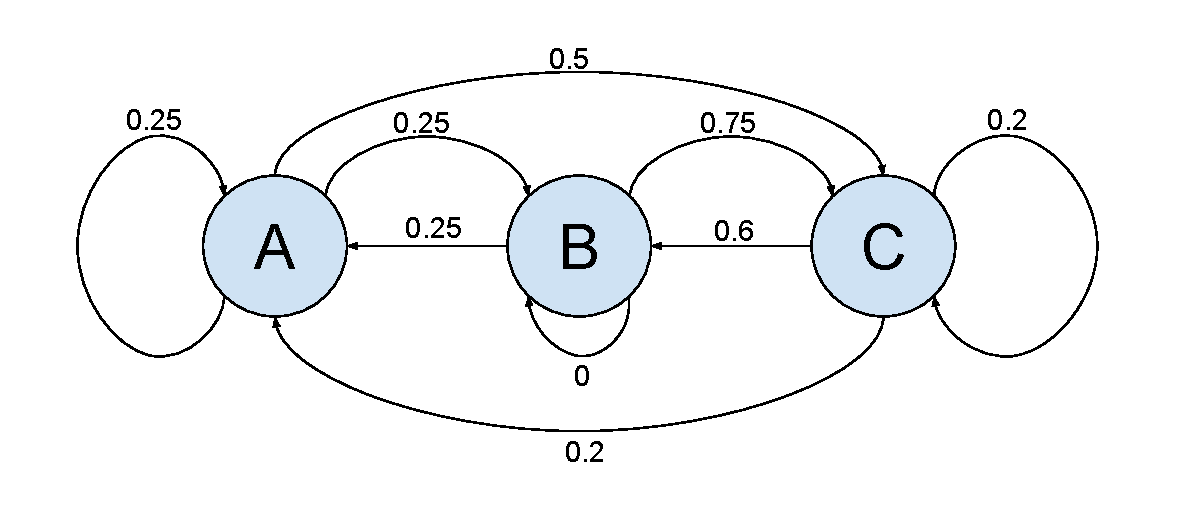
\includegraphics[width=1\textwidth]{MarkovChainExample}
	\caption{Example Markov Chain}
	\label{fig:Chain}
\end{figure}

\section{Haiku Constraint Problem}
With a dictionary of words to choose from, the haiku generation problem is easily represented as a constraint problem due to its rigid structure. Since each haiku is composed of three lines with a fixed syllable count, the problem can be broken down into three separate constraint problems. The task is then fill in each line with words that satisfy the total number of syllables required for each line.

\subsection{Counting Syllables}
There are multiple approaches we could have taken in determining the number of syllables in a word. We considered using a database loaded with an English dictionary. Dictionaries already have the words split up into syllables, so as long as the word exists in the dictionary then we would know exactly how many syllables it has. The issue with this approach is that it is not generalizable. Some dictionaries will not include a lot of words with various prefixes and suffixes. They also will not contain many slang words.

We instead outlined a general set of rules to determine syllables. These rules accurately determine the correct number of syllables in the majority of instances. The rules will not work in all cases. There is a large number of exceptions and corner cases making it difficult for the rules to be all encompassing, but they work for our purposes. In the context of these rules, y is considered as a vowel\cite{syllables}.
\begin{enumerate}
	\item If a vowel is preceded by a consonant, then increment the number of syllables.
	\item If an o is preceded by a vowel that is not an o, then increment the number of syllables.
	\item If there is an e at the end of a word preceded by a consonant, then increment the number of syllables if:
	\begin{itemize}
		\item The consonant is an l.
		\item The consonant is not an l and The letter that precedes the consonant is also a consonant.
	\end{itemize}
	\item Increment the number of syllables if the last three letters are "ing" and are preceded by a vowel.
\end{enumerate}

\begin{table}[H]
\begin{center}
	\begin{tabular}{| c | c |}
		\hline
		Word & Number of Syllables \\
		\hline
		biology & 4 \\
		\hline
		mile & 2 \\
		\hline
		fame & 1 \\
		\hline
		queueing & 2 \\
		\hline
	\end{tabular}
\caption{Words with syllables according to rules outlined}
\label{table:syllables}
\end{center}
\end{table}

In table \ref{table:syllables} biology has four syllables using rules 1 and 2. Mile has two syllables using rules 1 and 3. Fame has one syllable use rule 1. Queueing has two syllables according to rules 1 and 4. \comment{Needs citation}
\subsection{The Search Space}
Our search space was represented by a Markov chain where each variable is a node that contains the word it represents and the number of syllables it contains. The node is then linked to other nodes based on the relationships between the words represented in the nodes. These relationships are determined by the likelihood that one word is succeeded or proceeded by another based on the input file used to generate our dictionary.

To generate these relationships and ultimately the Markov chain, we require that the user provide a text file filled with sentences and phrases that get read in and the relationships between words in that file become the basis for our Markov chain. We treat each line in the input file independently from the previous, meaning that the last word of the first line will not have a relationship with the first word in the second. The parser starts each line by reading the first word and counting its syllables and adding it to the chain the second word is then read in and a connection from the first word to the second word is created and a counter of how many times the relationship appears is incremented. This process then repeats until the entire file has been read and converted to the Markov chain. At this point, instead of probabilities the relations between words has a count of how many times this relationship appears, so for each node in the chain we need to convert these into probabilities by summing the total number of relationships and dividing each count by this sum. The end result of parsing the file is a Markov chain that contains a node for every word in the file and a relationship for ever sequence of words that appears in the file.

Since space is at a premium in a haiku it may not be worth adding short and meaningless words such as prepositions. To accommodate for that a modifier flag has been built into the parser to ignore a list of user defined words. For example if a user wanted to ignore the word ``a'' the phrase ``eat a vegetable'' would omit ``a'' from the Markov chain and create a relationship instead between the words ``eat'' and ``vegetable.''

\section{Search Algorithms}
With the search space created the final step in generating a haiku was determining a way to navigate the search space We considered the trivial approach of choosing words at random from the Markov chain and adding them to the haiku where ever they may fit but odds are this would result in a lackluster haiku. Instead we decided to take three different approaches to navigating the space. The first being a slight spin on the trivial approach in that we choose our next word for the haiku from the previous word if possible. The second was a depth first approach in a way that would increase fluidity between words and hopefully generate a haiku that made sense. Finally we implemented a 

\subsection{Naive Search}
The first search method we attempted in our search space was trivial and consisted of picking a starting node in the chain and adding that word to the first available spot in any line of the haiku. The method then chose the next word from the chain as a child of the previous word and added it to any available space in the haiku that would not violate a syllable constraint. If the word could not be added it was ignored and used to generate the next word from it's children. If this approach ever reached a dead end in the chain it would pick a random node from the chain and continue from where it left off.

\begin{algorithm}[H]
	\caption{$Naive\_Search()$} \label{Naive}
	\begin{algorithmic}[1]
		\State Choose a random start node and set it to $current$
		\While{Haiku is not full}
			\State if possible, add $current$ to open line in haiku
			\If{$current$ has children}
				\State choose random $child$ from $current$
				\State $current = child$
			\Else
				\State Choose a random node and set it to $current$
			\EndIf
		\EndWhile
	\end{algorithmic}
\end{algorithm}

While this method works for generating valid Haiku's it's rarely any better than throwing random words into a haiku and hoping there is some meaning to the madness. To increase the likelihood that a haiku generated has a connection between each word in the line it is best to force words that are contiguous in the haiku to be connected in the Markov chain. We implemented depth first search and an iterative random walk method to accomplish this.

\subsection{Depth First Search}
One of the methods we used to navigate the search space and generate a Haiku was depth first search (DFS) with restarts. To accomplish this we utilized a two-way linked list where each node contained a Markov node and generated it's child randomly by weighting each of the Markov nodes children's probability to generate each line individually. To initialize the search we chose a random Markov node from our Markov chain and had our root list node point to this node. The algorithm then chose a child node from that Markov node and determined how many syllables the line of words would currently have and if we're still within the constraint it would repeat. If we have exactly the number of syllables we needed the code would return the line represented by this linked list starting from the root and ending at the child. If the child we chose would violate our constraints we retreated to the parent and would randomly choose a child that we had not yet visited from this node. If no children we're available we would retreat up another node. Finally if we are at the root node and there are no children available the code would restart and choose a new random starting position in the Markov chain.

\begin{algorithm}[H]
	\caption{$Depth\_First\_Search(n)$} \label{DFSB}
	\begin{algorithmic}[1]
		\State Choose an random $root$ node from the chain.
		\State $current = root$
		\While {$Syllables \neq n$}
			\If{Have not visited all possible children of $current$}
				\State Choose random unvisited $child$ of $current$
				\If{$child.syllables \leq n$}
					\State $current = child$
				\EndIf
			\Else
				\If{$current == root$}
					\Return $Depth\_First\_Search(n)$
				\Else
					\State $current$ = $parent$ of $current$
				\EndIf
			\EndIf
		\EndWhile
		\Return Line represented by linked list defined by $root$
	\end{algorithmic}
\end{algorithm}

This approach was then extended to try and maintain fluidity between lines. Instead of generating a random node for the starting position of the line we attempted to use a child of the last node from the previous line. If the child we chose was unable to produce a valid line for the haiku we chose a different child of the previous line's last node. If we had exhausted all the children then the algorithm opted to lose fluidity and generate a random starting node for this line.

\begin{algorithm}[H]
	\caption{$Depth\_First\_Search(node, n)$} \label{DFSB_WithStart}
	\begin{algorithmic}[1]
		\State $root = node$
		\State $current = root$
		\While {$Syllables \neq n$}
		\If{Have not visited all possible children of $current$}
		\State Choose random unvisited $child$ of $current$
		\If{$child.syllables \leq n$}
		\State $current = child$
		\EndIf
		\Else
		\If{$current == root$}
			\State {generate new $child$ from the $parent$ of $root$}
			\Return {$Depth\_First\_Search(child, n)$}
		\Else
		\State $current$ = $parent$ of $current$
		\EndIf
		\EndIf
		\EndWhile
		\Return Line represented by linked list defined by $root$
	\end{algorithmic}
\end{algorithm}



\subsection{Iterative Random Walk}

Iterative random walk leverages the naive approach in an iterative fashion to improve the quality of the generated haikus. The algorithm iteratively generates five and seven syllable lines starting from the same node in the Markov chain while noting the number of nodes visited. If the algorithm chooses lines that used the fewest number of nodes, then the line should have the closest thematic meaning to the root node. This is due to the assumption that nodes with nonzero probabilities are related thematically.

\begin{algorithm}[H]
	\caption{$IterativeRandomWalk(n)$} \label{IterativeRandomWalk}
	\begin{algorithmic}[1]
		\State Choose random node to be $root$
		\State $fiveLines$
		\State $sevenLines$
		\For 0 to $n$-1
			\State $line$, $steps$ = $RandomWalk(root, 5)$
			\State add $line$, $steps$ to $fiveLines$
			\State $line$, $steps$ = $RandomWalk(root, 7)$
			\State add $line$, $steps$ to $sevenLines$ 
		\EndFor
		\State sort $fiveLines$ by $steps$
		\State sort $sevenLines$ by $steps$
		\State $Haiku$
		\State add first two lines of $fiveLines$ to $Haiku$
		\State add first line of $sevenLines$ to $Haiku$
		\State return $Haiku$
	\end{algorithmic}
\end{algorithm}

\begin{algorithm}[H]
	\caption{$RandomWalk(root, j)$} \label{RandomWalk}
	\begin{algorithmic}[1]
		\State $steps$ = 0
		\State $syllables$ = 0
		\State $line$
		\State $current$ = $root$
		\While $syllables$ < $j$
			\If{$current.Syllables$ + $syllables$ <= $j$}
				$syllables$ = $syllables$ + $current.Syllables$
				\State add $current.word$ to $line$
			\EndIf
			\State choose random $child$ from $current$
			$current$ = $child$
			$steps$ = $steps$ + 1
		\EndWhile
		\State return $line$, $steps$
	\end{algorithmic}
\end{algorithm}

Iterative random walk first chooses a random node from the Markov chain to be the root node. During each iteration the algorithm performs a random walk through the Markov chain starting from the root node. At each step of the random walk, the word from the current node is added to a collection if adding that word does not exceed the maximum number of syllables. Once the maximum number of syllables is reached, the collection is then returned along with the number of nodes visited. Once all of the iterations have been completed, the algorithm chooses the two five syllable lines with the fewest nodes visited and the seven syllable line with the fewest nodes visited to construct a haiku. 

\section{Results}
To test our haiku generation approaches, we selected two different sets of training data. For the first set we chose the lyrics of the hip hop artist Aesop Rock. Matt Daniels analyzed the lyrics of various hip hop artists for their verbosity, and Aesop Rock was by far the most verbose\cite{Vocab}. We thought that his lyrics would provide enough variety and enough words to create a reasonably sized Markov chain. The other data set we chose was a selection of Shakespeare's works. Shakespeare was known for his vocabulary and has a large enough body of work to choose from.

To generate haikus we ran three trials. We ran the first trial using a selection from Aesop Rock. We ran the second trial using a selection from Shakespeare, and for the third we used both. For each trial we generated fifty haikus using each of the four approaches: Naive, DFS, DFS maintaining fluidity, and iterative random walk, and we selected a haiku to represent each algorithm. The number of iterations chosen for random walk was ten.

\begin{center}
\textbf{Trial One: Aesop Rock Lyrics}
\end{center}

\begin{figure}[H]
	\centering
	dry grays supplied raise \break
	fiery colossus dead tombs \break
	vibes blissful light
	\caption{Naive approach from Aesop Rock lyrics}
	\label{fig:NaiveAesop}
\end{figure}

\begin{figure}[H]
	\centering
	thieves received \break
	blue face through terrors of woe \break
	brain tripped beta
	\caption{DFS approach one from Aesop Rock lyrics}
	\label{fig:DFSOneAesop}
\end{figure}

\begin{figure}[H]
	\centering
	recording til fell \break
	through mite infested grillage \break
	awaited my game
	\caption{DFS approach two from Aesop Rock lyrics}
	\label{fig:DFSTwoAesop}
\end{figure}

\begin{figure}[H]
	\centering
	clash to conflicting \break
	clash to insanity dolls \break
	clash to emerge
	\caption{Iterative Random Walk from Aesop Rock lyrics}
		\label{fig:IRWAesop}
	\end{figure}
\begin{center}
\textbf{Trial Two: Shakespeare}
\end{center}

\begin{figure}[H]
	\centering
	leprosy i' faith \break
	o'ertake torn owner's \break
	tongue was sleeping
	\caption{Naive from Shakespeare}
	\label{fig:NaiveShakespeare}
\end{figure}

\begin{figure}[H]
	\centering
	cites virtuous \break
	admiring praise that i have \break
	driven on his name
	\caption{DFS approach one from Shakespeare}
	\label{fig:DPSOneShakespeare}
\end{figure}

\begin{figure}[H]
	\centering
	horror that i saw \break
	her audit though my uncle \break
	forest looks bleak air
	\caption{DFS approach two from Shakespeare}
	\label{fig:DFSTwoShakespeare}
\end{figure}

\begin{figure}[H]
	\centering
	slipper'd pantaloon \break
	penury these things without \break
	slipper'd pantaloon
	\caption{Iterative random walk from Shakespeare}
	\label{fig:IRWShakespeare}
\end{figure}

\begin{center}
	\textbf{Trial Three: Aesop Rock and Shakespeare}	
\end{center}

\begin{figure}[H]
	\centering
	lendin' bended dream \break
	be your praise confound thou \break
	distinction know'st
	\caption{Naive from Aesop Rock lyrics and Shakespeare}
	\label{fig:NaiveAesopShakespeare}
\end{figure}

\begin{figure}[H]
	\centering
	such contempt of truth \break
	disobedience he has \break
	demurely wake
	\caption{DFS approach one from Aesop Rock lyrics and Shakespeare}
	\label{fig:DFSOneAesopShakespeare}
\end{figure}

\begin{figure}[H]
	\centering
	over-goes my son \break
	was his mouth that i know more \break
	bright than i do look
	\caption{DFS approach two from Aesop Rock lyrics and Shakespeare}
	\label{fig:DFSTwoAesopShakespeare}
\end{figure}

\begin{figure}[H]
	\centering
	mood smell onions \break
	mood smell onions i say \break
	mood ring militant
	\caption{Iterative random walk from Aesop Rock lyrics and Shakespeare}
	\label{fig:IRWAesopShakespeare}
\end{figure}

The naive approach tended to produce haikus that made little sense. The DFS approaches were the most successful. We found quite a few in our collections that had similar thematic meaning to them. The iterative random walk tended to produce haikus with the same words repeated on multiple lines. Combining the texts of both Shakespeare and Aesop Rock had little success in combining themes. The dictionary of words used in each text were too different from each other, so the haikus ended up skewing towards Shakespeare or Aesop Rock depending on the initial node chosen.

\section{Future Work}
A final extension of the depth first search approach that is currently being implemented is to choose a starting node for the whole haiku and generate the entire haiku using just that node. Some haiku's generated by the approach that attempts to maintain consistency between lines would be valid in this sense but since any line could be restarted with a random node not all haiku's would be fluid throughout. This approach would need to be able to regenerate the previous line if the children of the last node cannot generate a new line. A suggested approach can be seen in algorithm \ref{Alg:DFSWhole}.

\begin{algorithm}[H]
	\caption{$Depth\_First\_Search\_Whole\_Haiku()$} \label{Alg:DFSWhole}
	\begin{algorithmic}[1]
		\State $LineMarker1$ = $Depth\_First\_Search(5)$
		\State $root$ = $LineMarker1.getRoot()$
		\State $LineMarker2$ = $Depth\_First\_Search(LineMarker1, 7)$
		\If {$LineMarker2 == null$} line could not be generated with parent node...
			\State Modify previous line so it ends on a different node, $newNode$
			\State $LineMarker1$ = $newNode$
			\State $LineMarker2$ = $Depth\_First\_Search(LineMarker1,7)$
		\EndIf
		\State $LineMarker3$ = $Deptt\_First\_Sarch(LineMarker2,5)$
		\If {$LineMarker3 == null$} line could not be generated with parent node...
			\State Modify previous line so it ends on a different node, $newNode$
			\State $LineMarker2$ = $newNode$
			\State $LineMarker3$ = $Depth\_First\_Search(LineMarker2,5)$
		\EndIf
		\State Haiku starts with $root$ and each $LineMarker$ shows where that line ends.
	\end{algorithmic}
\end{algorithm}

Furthermore, our methods generate valid haikus but a lot of them are lacking thematically or linguistically. More work could be done to improve the Markov chain and filter out words that don't have strong thematic relations with one another. Our user defined list of words to ignore in the file parser is a simple way we approached this problem. Another approach one could take towards this problem is to not allow lines to be valid if they end with words in a user defined list. For example: prohibit specific lines from ending with pronouns. Adding extra constraints to the problem could lead to better haikus being generated.

\section{Conclusion}
Generating poetry is quite the challenge for artificial intelligence. But by narrowing the scope from all forms of poetry to haikus we are able to take advantage of the rigid structure and lack of necessary rhyme scheme to begin to model the problem as solving one or a few constraint problems. Given a dictionary of words tied together via a Markov chain we were able to apply various search algorithms to solve these problems. Our implementations of naive search, depth first search, and shortest random walk each provided a way to generate haikus with varying, albeit random, fluidity and thematic contents. Naive search generated few haikus that made sense, depth first search provided the most successful in terms of making sense and flowing well, and shortest random walks provided poems that often sounded nice due to a clear repetition of words. However each search has it's drawbacks and not a single method is able to generate perfect haikus each time. Improvements to how the chain is built and building a list of rules for the haiku to further constrain the problem will further aid in generating better haikus.

\bibliography{mybib}
\bibliographystyle{plain}
\end{document}
